\documentclass[11pt, a4paper]{article}

\usepackage[utf8]{inputenc}
\usepackage[T1]{fontenc}
\usepackage[portuguese]{babel}
\usepackage[sfdefault]{roboto}
% Margem inferior ajustada para 1.5cm para caber o rodapé
\usepackage[top=7.5cm, headheight=7.5cm, bottom=1.3cm, footskip=0.5cm, left=1cm, right=1cm]{geometry}

% --- CARREGA O PACOTE DE IMAGEM PRIMEIRO ---
\usepackage{graphicx}

% --- CABEÇALHO E RODAPÉ EM TODAS AS PÁGINAS ---
\usepackage{fancyhdr}
\pagestyle{fancy}
\fancyhf{} 
\renewcommand{\headrulewidth}{0pt} 
\fancyhead[C]{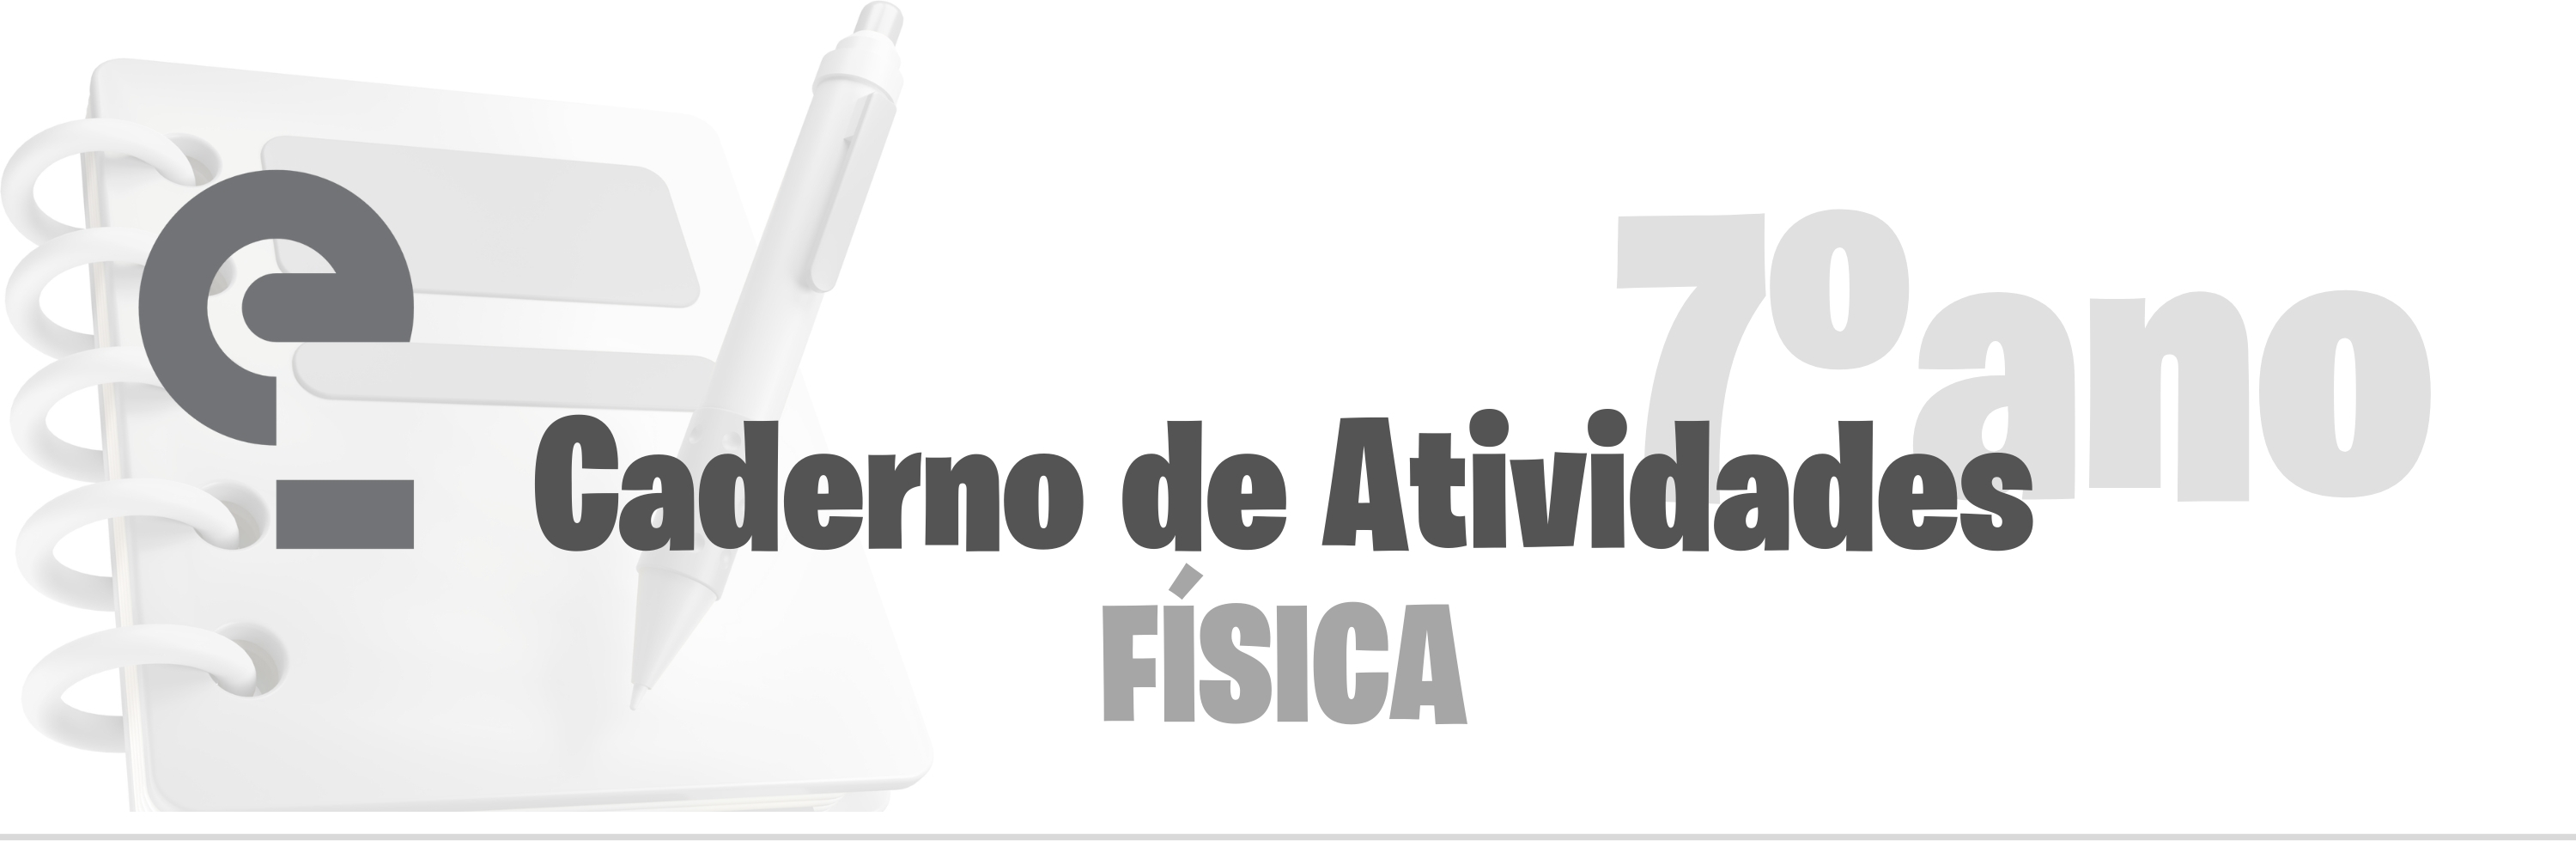
\includegraphics[width=\textwidth]{FISICA_7ANO.JPG}}
\fancyfoot[C]{Página \thepage} % Numeração centralizada (Use [R] se preferir à direita)

\usepackage{setspace}
\setstretch{1.15}
\usepackage{parskip}
\setlength{\parskip}{2pt}
\setlength{\parindent}{0pt}

\usepackage{amsmath, amsfonts, amssymb}
\usepackage{nccmath}
\usepackage{mathastext}
\usepackage{xcolor}
\definecolor{CorTitUm}{HTML}{FF6F61}
\definecolor{CorTitDois}{HTML}{FF6F61}
\definecolor{CorTitTres}{HTML}{658894}
\definecolor{CorLinha}{HTML}{B0B0B0}   

\usepackage{titlesec}
\titleformat{\section}{\color{CorTitUm}\fontsize{17}{20}\bfseries}{\thesection}{0em}{}
\titlespacing*{\section}{0pt}{5pt}{6pt} 
\titleformat{\subsection}{\color{CorTitDois}\fontsize{14}{16}\bfseries\raggedright\MakeUppercase}{\thesubsection}{0em}{}
\titlespacing*{\subsection}{0pt}{1pt}{5pt} 
\titleformat{\subsubsection}{\color{CorTitTres}\fontsize{12}{14}\bfseries\raggedright}{\thesubsubsection}{0em}{}
\titlespacing*{\subsubsection}{0pt}{-3pt}{1pt}

\usepackage{multicol}
\setlength{\columnsep}{1cm}
\setlength{\columnseprule}{0.5pt}
\def\columnseprulecolor{\color{CorLinha}}

% --- LIMITADOR DE IMAGENS ---
\usepackage{adjustbox}

\usepackage{tikz}
\usepackage{pgfplots}
\usepackage{circuitikz}
\usetikzlibrary{shadows, shapes.misc, positioning, calc}
\pgfplotsset{compat=1.18}

\begin{document}
\raggedcolumns
\section*{UNIDADE 6 - MÁQUINAS SIMPLES}
\begin{multicols*}{2}

\vspace{0cm} \noindent\textcolor{CorLinha}{\rule{\linewidth}{0.5pt}} \vspace{-0.2cm}
\subsection*{Capítulo 1: Fundamentos e Evolução Histórica}
\subsubsection*{QUESTÃO 01}
A história da humanidade está diretamente ligada à invenção de dispositivos que facilitam o trabalho. Desde a construção das pirâmides do Egito até os aquedutos romanos, a manipulação de forças foi essencial. Sobre o conceito físico de trabalho e a atuação das máquinas simples, analise as afirmativas a seguir e classifique-as como Verdadeiras (\textbf{V}) ou Falsas (\textbf{F}):

I. As máquinas simples reduzem a quantidade total de trabalho físico realizado para deslocar um objeto.\\[0.3cm]
II. Uma máquina simples pode alterar a direção da força aplicada, facilitando a execução de uma tarefa.\\[0.3cm]
III. O uso de um plano inclinado diminui a força necessária para elevar uma carga, mas exige que ela percorra uma distância maior.
\vspace{0cm} \noindent\textcolor{CorLinha}{\rule{\linewidth}{0.5pt}} \vspace{-0.2cm}
\subsubsection*{QUESTÃO 02}
Durante a Idade Média, o desenvolvimento de fortificações e armamentos de cerco, como as catapultas, exigiu um refinamento empírico da mecânica. Do ponto de vista da Física, explique qual é a principal vantagem mecânica obtida ao se utilizar um dispositivo que atua como multiplicador de força.
\vspace{0cm} \noindent\textcolor{CorLinha}{\rule{\linewidth}{0.5pt}} \vspace{-0.2cm}
\subsubsection*{QUESTÃO 03}
O esquema a seguir ilustra o princípio de funcionamento de uma catapulta clássica, onde uma força é aplicada em uma extremidade para lançar um projétil na outra.

\begin{center}
\begin{adjustbox}{max width=\linewidth}
\begin{tikzpicture}
% --- APLICANDO DROP SHADOW, CORES HEX E BORDAS ARREDONDADAS ---
\definecolor{madeira}{HTML}{8B5A2B}
\definecolor{metal}{HTML}{7F8C8D}
\definecolor{pedra}{HTML}{95A5A6}

% LAYER 1: Fundo (Chão)
\draw[drop shadow={opacity=0.15}, fill=gray!15, rounded corners=2pt, draw=none] (-3.5,-0.5) rectangle (3.5,0);

% LAYER 2: Ponto de apoio
\draw[drop shadow={opacity=0.2}, fill=metal, rounded corners=1pt] (-0.5,0) -- (0.5,0) -- (0,1) -- cycle;

% LAYER 3: Haste da alavanca
\draw[drop shadow={opacity=0.2}, fill=madeira, rounded corners=2pt, rotate around={15:(0,1)}] (-2.8,0.9) rectangle (2.8,1.1);

% LAYER 4: Carga (projétil)
\draw[drop shadow={opacity=0.2}, fill=pedra, rounded corners=3pt, rotate around={15:(0,1)}] (-2.6, 1.1) rectangle (-1.6, 1.9);
\node[rotate=15] at (-2.3, 2.1) [fill=white, inner sep=1pt] {\textbf{Projétil}};

% LAYER 5: Força aplicada
\draw[->, line width=1.5pt, draw=black] (2.2, 2.2) -- (2.2, 1) node[midway, right, fill=white, inner sep=2pt] {\textbf{F}};
\node at (0, -0.25) [fill=gray!15, inner sep=2pt] {\textbf{Apoio}};
\end{tikzpicture}
\end{adjustbox}
\end{center}

Considerando as posições da força motriz (\textbf{F}), do projétil (resistência) e do ponto de apoio geométrico, classifique o tipo de alavanca operada pelo mecanismo e justifique sua resposta.

\vspace{0cm} \noindent\textcolor{CorLinha}{\rule{\linewidth}{0.5pt}} \vspace{-0.2cm}
\subsubsection*{QUESTÃO 04}
A Revolução Industrial marcou a transição da manufatura artesanal para a produção mecanizada. Nesse contexto, rodas, eixos e polias foram amplamente combinados para formar engrenagens complexas nos teares mecânicos. Embora essas máquinas modernas fossem movidas a vapor, seus princípios operacionais ainda dependiam estritamente das máquinas simples. Demonstre, através de uma justificativa física, por que é impossível criar uma máquina que amplie simultaneamente a força aplicada e a velocidade de deslocamento sem fornecer energia externa.
\vspace{0cm} \noindent\textcolor{CorLinha}{\rule{\linewidth}{0.5pt}} \vspace{-0.2cm}
\subsubsection*{QUESTÃO 05}
(Estilo UNESP - Adaptada) As ferramentas utilizadas diariamente em residências e oficinas são, na sua grande maioria, aplicações diretas dos princípios físicos das máquinas simples estabelecidos desde a Antiguidade. Considere os seguintes instrumentos:
1. Uma tesoura de costura.
2. Um abridor de garrafas.
3. Uma maçaneta de porta convencional.

Os princípios físicos predominantes em cada um desses instrumentos correspondem, respectivamente, a:\\[0.3cm]
a) Alavanca interfixa, plano inclinado, roda e eixo.\\[0.3cm]
b) Alavanca interpotente, alavanca interfixa, polia.\\[0.3cm]
c) Alavanca interfixa, alavanca inter-resistente, roda e eixo.\\[0.3cm]
d) Plano inclinado, alavanca inter-resistente, polia fixa.\\[0.3cm]
e) Alavanca interpotente, plano inclinado, roda e eixo.
\vspace{0cm} \noindent\textcolor{CorLinha}{\rule{\linewidth}{0.5pt}} \vspace{-0.2cm}
\subsection*{Capítulo 2: Princípios Físicos (Alavancas, Polias e Planos)}
\subsubsection*{QUESTÃO 06}
Para manter o sistema em repouso perfeito na horizontal, um professor de física posicionou dois blocos maciços sobre uma prancha articulada, conforme o arranjo geométrico ilustrado a seguir.

\begin{center}
\begin{adjustbox}{max width=\linewidth}
\begin{tikzpicture}
% --- APLICANDO DROP SHADOW, CORES HEX E BORDAS ARREDONDADAS ---
\definecolor{base}{HTML}{2C3E50}
\definecolor{prancha}{HTML}{F39C12}
\definecolor{blocoA}{HTML}{2980B9}
\definecolor{blocoB}{HTML}{C0392B}

% LAYER 1: Chão e linhas de cota
\draw[fill=gray!10, draw=none] (-4,-1) rectangle (4, -0.5);
\draw[thick, color=gray!50] (-4,-0.5) -- (4,-0.5);

% LAYER 2: Apoio central
\draw[drop shadow={opacity=0.2}, fill=base, rounded corners=1pt] (-0.5,-0.5) -- (0.5,-0.5) -- (0,0.5) -- cycle;

% LAYER 3: Prancha
\draw[drop shadow={opacity=0.2}, fill=prancha, rounded corners=2pt] (-3.5,0.5) rectangle (3.5,0.7);

% LAYER 4: Blocos com massas
\draw[drop shadow={opacity=0.2}, fill=blocoA, rounded corners=2pt] (-3,0.7) rectangle (-2,1.7) node[pos=.5, text=white] {\textbf{60 kg}};
\draw[drop shadow={opacity=0.2}, fill=blocoB, rounded corners=2pt] (1.5,0.7) rectangle (2.5,1.7) node[pos=.5, text=white] {\textbf{m}};

% LAYER 5: Cotas dimensionais com máscara de fundo branco
\draw[<->, >=stealth, thick] (-2.5, 2.3) -- (0, 2.3) node[midway, fill=white, inner sep=2pt] {\textbf{2,0 m}};
\draw[<->, >=stealth, thick] (0, 2.3) -- (2, 2.3) node[midway, fill=white, inner sep=2pt] {\textbf{3,0 m}};
\draw[dashed, color=gray!80] (-2.5, 1.7) -- (-2.5, 2.5);
\draw[dashed, color=gray!80] (0, 0.5) -- (0, 2.5);
\draw[dashed, color=gray!80] (2, 1.7) -- (2, 2.5);
\end{tikzpicture}
\end{adjustbox}
\end{center}
Determine o valor numérico da massa \textbf{m} do bloco vermelho para que a condição de equilíbrio estático rotacional seja satisfeita.
\vspace{0cm} \noindent\textcolor{CorLinha}{\rule{\linewidth}{0.5pt}} \vspace{-0.2cm}
\subsubsection*{QUESTÃO 07}
Em um canteiro de obras, um operário precisa erguer uma caixa de ferramentas utilizando um sistema de içamento acoplado ao teto do andaime, como esquematizado na figura abaixo.
\begin{center}
\begin{adjustbox}{max width=\linewidth}
\begin{tikzpicture}
% --- APLICANDO DROP SHADOW, CORES HEX E BORDAS ARREDONDADAS ---
\definecolor{teto}{HTML}{7F8C8D}
\definecolor{corda}{HTML}{34495E}
\definecolor{polia}{HTML}{BDC3C7}
\definecolor{carga}{HTML}{8E44AD}

% LAYER 1: Teto
\draw[fill=teto, drop shadow={opacity=0.2}] (-2,4) rectangle (2,4.3);

% LAYER 2: Polias e suportes
\draw[fill=polia, drop shadow={opacity=0.15}] (1,3) circle (0.4);
\draw[fill=gray!80] (1,3) circle (0.1);
\draw[thick, color=teto] (1,3) -- (1,4); % CORRIGIDO de "base" para "teto"

\draw[fill=polia, drop shadow={opacity=0.15}] (-1,2) circle (0.4);
\draw[fill=gray!80] (-1,2) circle (0.1);

% LAYER 3: Cabeamento (Cordas)
\draw[thick, color=corda] (-1.4,4) -- (-1.4,2); 
\draw[thick, color=corda] (-0.6,2) -- (0.6,3); 
\draw[thick, color=corda, ->, >=stealth] (1.4,3) -- (1.4,1) node[below, fill=white, inner sep=2pt] {\textbf{F}};

% LAYER 4: Carga
\draw[thick, color=teto] (-1,2) -- (-1,1.2); % CORRIGIDO de "base" para "teto"
\draw[fill=carga, drop shadow={opacity=0.2}, rounded corners=2pt] (-1.6,0.2) rectangle (-0.4,1.2) node[pos=.5, text=white] {\textbf{800 N}};
\end{tikzpicture}
\end{adjustbox}
\end{center}

Com base na associação de roldanas empregada, calcule o valor da força motriz ideal \textbf{F} que o operário deve aplicar verticalmente para baixo, a fim de içar a carga com velocidade constante.
\vspace{0cm} \noindent\textcolor{CorLinha}{\rule{\linewidth}{0.5pt}} \vspace{-0.2cm}
\subsubsection*{QUESTÃO 08}
A alavanca é composta basicamente por uma barra rígida e um ponto de apoio. Dependendo da posição do ponto de apoio em relação à força potente e à força resistente, ela recebe uma classificação específica. Considere os seguintes instrumentos de uso comum:
I. Um quebra-nozes mecânico.
II. Uma pinça de sobrancelha.
III. Uma gangorra de parque.

Identifique e descreva a classificação física (interfixa, interpotente ou inter-resistente) de cada um dos instrumentos listados.
\vspace{0cm} \noindent\textcolor{CorLinha}{\rule{\linewidth}{0.5pt}} \vspace{-0.2cm}
\subsubsection*{QUESTÃO 09}
A rampa de acesso ao setor de logística de um armazém foi projetada com medidas específicas para minimizar o esforço dos funcionários, conforme a representação geométrica a seguir.

\begin{center}
\begin{adjustbox}{max width=\linewidth}
\begin{tikzpicture}
% --- APLICANDO DROP SHADOW E BORDAS ARREDONDADAS ---
\definecolor{rampa}{HTML}{BDC3C7}
\definecolor{caixa}{HTML}{D35400}
\definecolor{chao}{HTML}{95A5A6}

% LAYER 1: Estrutura da Rampa
\draw[fill=rampa, drop shadow={opacity=0.15}, draw=gray!70] (0,0) -- (5,0) -- (5,2.5) -- cycle;
\draw[thick, color=chao] (-1,0) -- (6,0);

% LAYER 2: Cotas dimensionais
\draw[thick, color=black] (5,0) -- (5,2.5) node[midway, right, fill=white, inner sep=2pt] {\textbf{2,0 m}};
\draw[thick, color=black] (0,0) -- (5,2.5) node[pos=0.1, above right, fill=white, inner sep=2pt, sloped] {\textbf{10,0 m}};

% LAYER 3: Objeto na rampa
\draw[fill=caixa, drop shadow={opacity=0.2}, rounded corners=1pt, rotate around={26.5:(2,1)}] (2,1) rectangle (3.3,1.6) node[pos=.5, text=white, rotate=26.5] {\textbf{500 N}};

% LAYER 4: Vetor Força Motriz
\draw[->, >=stealth, line width=1.2pt, rotate around={26.5:(2,1)}] (3.3, 1.3) -- (4, 1.3) node[above, sloped, fill=white, inner sep=1pt] {\textbf{F}};
\end{tikzpicture}
\end{adjustbox}
\end{center}

Sem considerar as perdas por atrito, aplique o princípio da vantagem mecânica do plano inclinado e determine o valor da força \textbf{F} necessária para empurrar o objeto uniformemente até o topo.
\vspace{0cm} \noindent\textcolor{CorLinha}{\rule{\linewidth}{0.5pt}} \vspace{-0.2cm}
\subsubsection*{QUESTÃO 10}
(Estilo ENEM - Adaptada) A combinação de uma roda rigidamente presa a um eixo concêntrico constitui uma máquina simples cujo objetivo é transferir torque e amplificar forças rotacionais. Nas aplicações práticas modernas, essa mecânica é vital. Sobre a "roda e eixo", julgue as afirmativas a seguir assinalando Verdadeiro (\textbf{V}) ou Falso (\textbf{F}):

I. Quando aplicamos força na extremidade do volante de um automóvel (roda), a força transferida para a barra de direção (eixo) é menor do que a aplicada.\\[0.3cm]
II. O diâmetro maior da maçaneta de uma porta em relação ao seu eixo interno garante uma vantagem mecânica que facilita o destravamento da fechadura.\\[0.3cm]
III. Se a força motriz for aplicada no eixo em vez de na roda (como nos pneus traseiros de um carro), haverá um ganho de velocidade periférica em sacrifício da força.
\vspace{0cm} \noindent\textcolor{CorLinha}{\rule{\linewidth}{0.5pt}} \vspace{-0.2cm}
\subsubsection*{QUESTÃO 11}
Sistemas compostos por múltiplas polias móveis, conhecidos como talhas exponenciais, são projetados para levantar cargas massivas em estaleiros e portos. O sistema esquematizado opera içando um contêiner sob tensão contínua.

\begin{center}
\begin{adjustbox}{max width=\linewidth}
\begin{tikzpicture}
% --- APLICANDO DROP SHADOW, CORES HEX E BORDAS ARREDONDADAS ---
\definecolor{teto}{HTML}{34495E}
\definecolor{poliaF}{HTML}{95A5A6}
\definecolor{poliaM}{HTML}{F1C40F}
\definecolor{bloco}{HTML}{E74C3C}

% LAYER 1: Teto suporte
\draw[fill=teto, drop shadow={opacity=0.2}] (-2,5) rectangle (3,5.3);

% LAYER 2: Polia Fixa
\draw[fill=poliaF, drop shadow={opacity=0.15}] (2,4) circle (0.4);
\draw[fill=white] (2,4) circle (0.1);
\draw[thick] (2,4) -- (2,5);

% LAYER 3: Polias Móveis
\draw[fill=poliaM, drop shadow={opacity=0.15}] (0.5,3) circle (0.4);
\draw[fill=white] (0.5,3) circle (0.1);

\draw[fill=poliaM, drop shadow={opacity=0.15}] (-1,2) circle (0.4);
\draw[fill=white] (-1,2) circle (0.1);

% LAYER 4: Cordas (Talha Exponencial)
% Corda da Polia 1 (inferior)
\draw[thick] (-1.4,5) -- (-1.4,2); 
\draw[thick] (-0.6,2) -- (-0.6,3); % Conecta ao eixo da proxima
\draw[thick] (-0.6,3) -- (0.5,3); % Suporte horizontal adaptado pro eixo
% Corda da Polia 2 (meio)
\draw[thick] (0.1,5) -- (0.1,3);
\draw[thick] (0.9,3) -- (0.9,4);
\draw[thick] (0.9,4) -- (2,4);
% Corda final (puxada)
\draw[thick] (1.6,5) -- (1.6,4);
\draw[thick, ->, >=stealth] (2.4,4) -- (2.4,2) node[below, fill=white, inner sep=2pt] {\textbf{F}};

% LAYER 5: Carga pesada acoplada a polia móvel 1
\draw[thick] (-1,2) -- (-1,1);
\draw[fill=bloco, drop shadow={opacity=0.2}, rounded corners=2pt] (-1.8,0) rectangle (-0.2,1) node[pos=.5, text=white] {\textbf{1600 N}};
\end{tikzpicture}
\end{adjustbox}
\end{center}

Neste arranjo contendo exatamente duas polias móveis e uma fixa, calcule a intensidade da força \textbf{F} necessária para equilibrar a carga.

\vspace{0cm} \noindent\textcolor{CorLinha}{\rule{\linewidth}{0.5pt}} \vspace{-0.2cm}
\subsubsection*{QUESTÃO 12}
Uma das aplicações mais eficientes da associação entre rodas e eixos pode ser observada no sistema de marchas (coroa e catraca) de uma bicicleta moderna. Explique o que ocorre fisicamente com a velocidade da bicicleta e com a força exigida do ciclista quando a corrente é mudada de uma catraca pequena para uma catraca traseira de raio muito maior.
\vspace{0cm} \noindent\textcolor{CorLinha}{\rule{\linewidth}{0.5pt}} \vspace{-0.2cm}
\subsubsection*{QUESTÃO 13}
A necessidade de elevar materiais pesados em construções civis popularizou o uso de polias. Um mestre de obras montou o esquema ilustrado abaixo, associando uma roldana fixa e uma móvel para erguer um bloco de cimento.

\begin{center}
\begin{adjustbox}{max width=\linewidth}
\begin{tikzpicture}
% --- APLICANDO DROP SHADOW, CORES HEX E BORDAS ARREDONDADAS ---
\definecolor{viga}{HTML}{2C3E50}
\definecolor{roldana}{HTML}{7F8C8D}
\definecolor{cimento}{HTML}{95A5A6}
\definecolor{cordame}{HTML}{E67E22}

% LAYER 1: Viga superior
\draw[fill=viga, drop shadow={opacity=0.2}] (-2,4) rectangle (2,4.3);

% LAYER 2: Roldanas (Fixa e Móvel)
\draw[fill=roldana, drop shadow={opacity=0.15}] (1,3) circle (0.4);
\draw[fill=white] (1,3) circle (0.1);
\draw[thick, color=viga] (1,3) -- (1,4); % Eixo da fixa

\draw[fill=roldana, drop shadow={opacity=0.15}] (-1,2) circle (0.4);
\draw[fill=white] (-1,2) circle (0.1);

% LAYER 3: Cordame
\draw[thick, color=cordame] (-1.4,4) -- (-1.4,2); 
\draw[thick, color=cordame] (-0.6,2) -- (0.6,3); 
\draw[thick, color=cordame, ->, >=stealth] (1.4,3) -- (1.4,1) node[below, fill=white, inner sep=2pt] {\textbf{F}};

% LAYER 4: Bloco de cimento
\draw[thick, color=viga] (-1,2) -- (-1,1.2);
\draw[fill=cimento, drop shadow={opacity=0.2}, rounded corners=2pt] (-1.5,0.2) rectangle (-0.4,1.2) node[pos=.5, text=black] {\textbf{500 N}};
\end{tikzpicture}
\end{adjustbox}
\end{center}

Determine o valor da força motriz \textbf{F} que o operário deverá aplicar na extremidade livre da corda para manter o bloco de cimento em equilíbrio estático no ar.
\vspace{0cm} \noindent\textcolor{CorLinha}{\rule{\linewidth}{0.5pt}} \vspace{-0.2cm}
\subsubsection*{QUESTÃO 14}
O uso de planos inclinados em estradas de montanha é uma aplicação direta da física para permitir que veículos alcancem grandes altitudes. Sobre a vantagem mecânica do plano inclinado, julgue as afirmativas a seguir com Verdadeiro (\textbf{V}) ou Falso (\textbf{F}):

I. Quanto mais extensa (comprida) for a rampa para atingir uma mesma altura, menor será a força necessária para subir o veículo.\\[0.3cm]
II. O plano inclinado reduz o trabalho total realizado pelo motor do carro, pois encurta a distância do trajeto.\\[0.3cm]
III. A força motriz necessária para empurrar um objeto rampa acima é diretamente proporcional à inclinação; rampas mais íngremes exigem mais força.
\vspace{0cm} \noindent\textcolor{CorLinha}{\rule{\linewidth}{0.5pt}} \vspace{-0.2cm}
\subsubsection*{QUESTÃO 15}
O carrinho de mão é uma das invenções mais geniais da mecânica clássica, operando como uma alavanca que facilita o transporte de cargas pesadas por uma única pessoa. O diagrama abaixo detalha as posições do eixo da roda, do centro de massa da carga e dos puxadores.

\begin{center}
\begin{adjustbox}{max width=\linewidth}
\begin{tikzpicture}
% --- APLICANDO DROP SHADOW, CORES HEX E BORDAS ARREDONDADAS ---
\definecolor{metal}{HTML}{34495E}
\definecolor{roda}{HTML}{2C3E50}
\definecolor{cargacaixa}{HTML}{D35400}

% LAYER 1: Solo e Roda (Ponto de Apoio)
\draw[thick, color=gray!50] (-1,0) -- (6,0);
\draw[fill=roda, drop shadow={opacity=0.2}] (0,0.5) circle (0.5);
\draw[fill=white] (0,0.5) circle (0.1) node[below=4pt, fill=white, inner sep=1pt] {\textbf{A}};

% LAYER 2: Estrutura do carrinho
\draw[thick, line width=2pt, color=metal] (0,0.5) -- (4,1.5);
\draw[thick, line width=2pt, color=metal] (4,1.5) -- (5,1.5) node[right] {\textbf{C}};

% LAYER 3: Carga
\draw[fill=cargacaixa, drop shadow={opacity=0.2}, rounded corners=3pt] (0.8, 1) -- (2.8, 1.5) -- (3, 2.5) -- (1, 2) -- cycle;
\node[fill=white, inner sep=1pt, rounded corners=1pt] at (2, 1.7) {\textbf{B (Carga)}};

% LAYER 4: Forças e Cotas
\draw[->, >=stealth, line width=1.2pt, color=black] (5,1.5) -- (5,2.5) node[above, fill=white, inner sep=1pt] {\textbf{F}};
\draw[->, >=stealth, line width=1.2pt, color=black] (2, 1.4) -- (2, 0.5) node[below, fill=white, inner sep=1pt] {\textbf{800 N}};

\draw[<->, >=stealth, dashed] (0, -0.5) -- (2, -0.5) node[midway, fill=white, inner sep=2pt] {\textbf{0,5 m}};
\draw[<->, >=stealth, dashed] (2, -0.5) -- (5, -0.5) node[midway, fill=white, inner sep=2pt] {\textbf{1,0 m}};
\draw[dashed, color=gray!80] (0,0) -- (0,-0.7);
\draw[dashed, color=gray!80] (2,0.5) -- (2,-0.7);
\draw[dashed, color=gray!80] (5,1.5) -- (5,-0.7);
\end{tikzpicture}
\end{adjustbox}
\end{center}

Sabendo que o carrinho atua como uma alavanca inter-resistente, calcule a força motriz \textbf{F} que o operador deve aplicar verticalmente para cima no ponto \textbf{C} para conseguir suspender o sistema e iniciar o transporte.
\vspace{0cm} \noindent\textcolor{CorLinha}{\rule{\linewidth}{0.5pt}} \vspace{-0.2cm}
\subsubsection*{QUESTÃO 16}
(Estilo FUVEST - Adaptada) Para carregar um cofre pesado de \textbf{1200 N} na carroceria de um caminhão que está a \textbf{1,5 m} de altura do solo, os entregadores utilizam uma prancha de madeira lisa atuando como plano inclinado. A prancha possui \textbf{4,5 m} de comprimento total. Desprezando qualquer força de atrito entre o cofre e a prancha, determine qual será a força constante, paralela à rampa, que os entregadores precisarão aplicar para empurrar o cofre de forma equilibrada até o topo. Demonstre seu raciocínio através da proporção linear entre as distâncias.
\vspace{0cm} \noindent\textcolor{CorLinha}{\rule{\linewidth}{0.5pt}} \vspace{-0.2cm}
\subsubsection*{QUESTÃO 17}
Durante uma aula prática no parquinho da escola, um professor de física pediu que dois alunos de massas diferentes se sentassem em uma gangorra (alavanca interfixa) de forma a mantê-la perfeitamente na horizontal, desafiando a intuição das crianças.

\begin{center}
\begin{adjustbox}{max width=\linewidth}
\begin{tikzpicture}
% --- APLICANDO DROP SHADOW, CORES HEX E BORDAS ARREDONDADAS ---
\definecolor{pedestal}{HTML}{16A085}
\definecolor{madeira}{HTML}{F39C12}
\definecolor{alunoA}{HTML}{8E44AD}
\definecolor{alunoB}{HTML}{2980B9}

% LAYER 1: Chão e Pedestal
\draw[fill=gray!15, draw=none] (-4.5,-0.5) rectangle (4.5,0);
\draw[thick, color=gray!50] (-4.5,0) -- (4.5,0);
\draw[fill=pedestal, drop shadow={opacity=0.2}, rounded corners=1pt] (-0.5,0) -- (0.5,0) -- (0,1) -- cycle;

% LAYER 2: Prancha da gangorra
\draw[fill=madeira, drop shadow={opacity=0.2}, rounded corners=2pt] (-4,1) rectangle (4,1.2);

% LAYER 3: Alunos (Blocos representativos)
\draw[fill=alunoA, drop shadow={opacity=0.2}, rounded corners=2pt] (-3.5,1.2) rectangle (-2.5,2.2) node[pos=.5, text=white] {\textbf{30 kg}};
\draw[fill=alunoB, drop shadow={opacity=0.2}, rounded corners=2pt] (1.5,1.2) rectangle (2.5,2.7) node[pos=.5, text=white] {\textbf{45 kg}};

% LAYER 4: Cotas de distância
\draw[<->, >=stealth, thick] (-3, 2.8) -- (0, 2.8) node[midway, fill=white, inner sep=2pt] {\textbf{1,8 m}};
\draw[<->, >=stealth, thick] (0, 2.8) -- (2, 2.8) node[midway, fill=white, inner sep=2pt] {\textbf{X}};
\draw[dashed, color=gray!80] (-3, 2.2) -- (-3, 3.0);
\draw[dashed, color=gray!80] (0, 1.2) -- (0, 3.0);
\draw[dashed, color=gray!80] (2, 2.7) -- (2, 3.0);
\end{tikzpicture}
\end{adjustbox}
\end{center}

Aplicando o princípio do equilíbrio das alavancas, determine a distância \textbf{X} que o aluno mais pesado (45 kg) deve ficar do eixo central para garantir que a gangorra não tombe para nenhum dos lados.
\vspace{0cm} \noindent\textcolor{CorLinha}{\rule{\linewidth}{0.5pt}} \vspace{-0.2cm}
\subsubsection*{QUESTÃO 18}
Poços artesianos rústicos frequentemente utilizam um sistema de manivela acoplado a um tambor cilíndrico para içar baldes de água do fundo. Esse mecanismo é a clássica representação física da máquina simples conhecida como "roda e eixo". Se o tambor cilíndrico (onde a corda se enrola) possui um raio de \textbf{10 cm} e a haste da manivela possui um braço de alavanca de \textbf{40 cm}, explique fisicamente por que é muito mais fácil puxar um balde pesado de água girando a manivela do que puxando a corda diretamente com as mãos.
\vspace{0cm} \noindent\textcolor{CorLinha}{\rule{\linewidth}{0.5pt}} \vspace{-0.2cm}
\subsubsection*{QUESTÃO 19}
(Estilo UNESP - Adaptada) Para remover o motor de um automóvel durante uma manutenção pesada, um mecânico opta por utilizar uma talha manual complexa. O arranjo físico escolhido por ele consiste em uma associação de fios ideais contendo 1 polia fixa presa ao teto da oficina e 3 polias móveis encadeadas livremente. Sabendo que o peso total do motor é de \textbf{1600 N}, a força ideal contínua que o mecânico precisa aplicar na ponta da corda para manter o motor suspenso é de:\\[0.3cm]
a) $ 1600 \text{ N} $\\[0.3cm]
b) $ 800 \text{ N} $\\[0.3cm]
c) $ 400 \text{ N} $\\[0.3cm]
d) $ 200 \text{ N} $\\[0.3cm]
e) $ 100 \text{ N} $

\vspace{0cm} \noindent\textcolor{CorLinha}{\rule{\linewidth}{0.5pt}} \vspace{-0.2cm}
\subsection*{Capítulo 3: Soluções Práticas e Aplicações Cotidianas}
\subsubsection*{QUESTÃO 20}
A chave de fenda é uma ferramenta essencial que pode atuar como duas máquinas simples distintas dependendo de como é usada. Quando a utilizamos para forçar a abertura da tampa de uma lata de tinta, ela age como uma alavanca. Porém, quando a giramos para apertar um parafuso, ela atua pelo princípio de roda e eixo. Considere duas chaves de fenda de mesmo comprimento, mas uma possui o cabo (empunhadura) muito mais grosso (maior diâmetro) que a outra. Qual das duas chaves exigirá menos esforço físico do trabalhador para girar um parafuso enferrujado? Justifique sua escolha com base nos princípios físicos da vantagem mecânica.
\vspace{0cm} \noindent\textcolor{CorLinha}{\rule{\linewidth}{0.5pt}} \vspace{-0.2cm}
\subsubsection*{QUESTÃO 21}
O próprio corpo humano é um complexo sistema de máquinas simples. Ao segurarmos um objeto pesado com a mão e dobrarmos o cotovelo, o sistema osso-músculo atua exatamente como uma alavanca. O diagrama ilustra as forças em ação no antebraço.

\begin{center}
\begin{adjustbox}{max width=\linewidth}
\begin{tikzpicture}
% --- APLICANDO DROP SHADOW, CORES HEX E BORDAS ARREDONDADAS ---
\definecolor{pele}{HTML}{F5CBA7}
\definecolor{musculo}{HTML}{E74C3C}
\definecolor{peso}{HTML}{7F8C8D}

% LAYER 1: Braço superior e antebraço (Formas simplificadas)
\draw[fill=pele, drop shadow={opacity=0.15}, rounded corners=4pt] (-1,0) rectangle (0,4); % Braço
\draw[fill=pele, drop shadow={opacity=0.15}, rounded corners=4pt] (-0.5,-0.5) rectangle (5,0.5); % Antebraço

% LAYER 2: Articulação e Músculo
\draw[fill=white, thick] (0,0) circle (0.2) node[below=6pt, fill=white, inner sep=1pt] {\textbf{Articulação (Apoio)}};
\draw[fill=musculo, rounded corners=3pt, opacity=0.8] (-0.2, 3) to[out=-20, in=120] (1, 0.4) to[out=180, in=-60] (-0.8, 2) -- cycle;

% LAYER 3: Peso na mão
\draw[fill=peso, drop shadow={opacity=0.2}, rounded corners=2pt] (4.5,-0.2) rectangle (5.5,0.8) node[pos=.5, text=white] {\textbf{P}};

% LAYER 4: Vetores e Cotas
\draw[->, >=stealth, line width=1.5pt, color=black] (1,0.5) -- (1,2) node[above, fill=white, inner sep=2pt] {\textbf{F (Bíceps)}};
\draw[->, >=stealth, line width=1.5pt, color=black] (5,0.2) -- (5,-1.5) node[below, fill=white, inner sep=2pt] {\textbf{40 N}};

\draw[<->, >=stealth, dashed] (0, -1) -- (1, -1) node[midway, fill=white, inner sep=1pt] {\textbf{4 cm}};
\draw[<->, >=stealth, dashed] (1, -1) -- (5, -1) node[midway, fill=white, inner sep=1pt] {\textbf{36 cm}};
\draw[dashed, color=gray!80] (0,-0.3) -- (0,-1.2);
\draw[dashed, color=gray!80] (1,-0.5) -- (1,-1.2);
\draw[dashed, color=gray!80] (5,-0.5) -- (5,-1.2);
\end{tikzpicture}
\end{adjustbox}
\end{center}

Neste arranjo (onde a força potente está entre o apoio e a resistência), o antebraço atua como uma alavanca interpotente. Calcule a força \textbf{F} que o músculo bíceps deve exercer para equilibrar o peso de \textbf{40 N} sustentado pela mão.
\vspace{0cm} \noindent\textcolor{CorLinha}{\rule{\linewidth}{0.5pt}} \vspace{-0.2cm}
\subsubsection*{QUESTÃO 22}
A invenção de ferramentas especializadas visou contornar limitações físicas do ser humano. Analise as afirmativas abaixo sobre ferramentas comuns e assinale Verdadeiro (\textbf{V}) ou Falso (\textbf{F}):

I. Uma pinça de depilação é uma alavanca interpotente, projetada não para multiplicar a força, mas sim para fornecer controle fino e precisão na movimentação.\\[0.3cm]
II. O quebra-nozes atua como uma alavanca inter-resistente, pois a noz (resistência) é esmagada entre o eixo (dobradiça) e a força aplicada pelas mãos.\\[0.3cm]
III. Um alicate de corte é ineficiente para partir fios de aço espessos, pois atua como uma alavanca interpotente que divide a força aplicada pelo trabalhador.
\vspace{0cm} \noindent\textcolor{CorLinha}{\rule{\linewidth}{0.5pt}} \vspace{-0.2cm}
\subsubsection*{QUESTÃO 23}
Para garantir a acessibilidade em calçadas, a norma brasileira NBR 9050 exige que rampas para cadeirantes não excedam uma proporção física limite para que o esforço não seja excessivo. A figura representa o projeto de uma dessas rampas.

\begin{center}
\begin{adjustbox}{max width=\linewidth}
\begin{tikzpicture}
% --- APLICANDO DROP SHADOW, CORES HEX E BORDAS ARREDONDADAS ---
\definecolor{concreto}{HTML}{BDC3C7}
\definecolor{piso}{HTML}{7F8C8D}

% LAYER 1: Chao e rampa
\draw[thick, color=piso] (-1,0) -- (9,0);
\draw[fill=concreto, drop shadow={opacity=0.15}, draw=gray!70] (0,0) -- (8,0) -- (8,0.8) -- cycle;

% LAYER 2: Cadeirante simplificado (Icone)
\draw[fill=white, thick] (2, 0.45) circle (0.2); % roda
\draw[thick, rounded corners=1pt] (2,0.45) -- (2, 0.9) -- (2.3, 0.9); % banco
\fill (2.1, 1.1) circle (0.1); % cabeça

% LAYER 3: Cotas com máscara
\draw[<->, >=stealth, thick] (8.3, 0) -- (8.3, 0.8) node[midway, right, fill=white, inner sep=1pt] {\textbf{0,6 m (Altura)}};
\draw[<->, >=stealth, thick] (0, -0.5) -- (8, -0.5) node[midway, fill=white, inner sep=2pt] {\textbf{D (Comprimento horizontal)}};
\draw[dashed, color=gray!80] (0,0) -- (0,-0.7);
\draw[dashed, color=gray!80] (8,0) -- (8,-0.7);
\end{tikzpicture}
\end{adjustbox}
\end{center}

Se a legislação local estabelece que a vantagem mecânica ideal (desprezando o atrito) deve exigir que a força aplicada seja de apenas $ \mfrac{1}{10} $ do peso total da cadeira de rodas e seu ocupante, qual deve ser o comprimento \textbf{D} aproximado da rampa para vencer a altura de \textbf{0,6 m}? *(Dica: Pense na proporção direta entre os comprimentos e as forças).*
\vspace{0cm} \noindent\textcolor{CorLinha}{\rule{\linewidth}{0.5pt}} \vspace{-0.2cm}
\subsubsection*{QUESTÃO 24}
(Estilo ENEM - Oficial Adaptada) Um ciclista experiente sabe que o sistema de transmissão de sua bicicleta (coroa, corrente e catraca) funciona como um conjunto de roldanas acopladas por uma correia. Ao encarar uma subida muito íngreme, o ciclista decide acionar o câmbio para tornar a pedalada mais "leve". Do ponto de vista das máquinas simples (roda e eixo/polias), a pedalada se torna mais leve, exigindo menor força das pernas, quando a corrente passa a ligar:

a) Uma coroa grande dianteira a uma catraca pequena traseira, garantindo maior velocidade da roda.
b) Uma coroa pequena dianteira a uma catraca grande traseira, maximizando a vantagem mecânica de torque.\\[0.1cm]
c) Polias de raios exatamente iguais, cancelando o atrito da corrente.\\[0.1cm]
d) O eixo central diretamente à roda traseira, eliminando o uso da corrente transmissora.\\[0.1cm]
e) Uma catraca traseira cujo raio seja menor que o eixo central da roda, invertendo a força.
\vspace{0cm} \noindent\textcolor{CorLinha}{\rule{\linewidth}{0.5pt}} \vspace{-0.2cm}
\subsubsection*{QUESTÃO 25}
Chegamos ao último desafio do seu treinamento em mecânica básica. Você foi contratado como consultor técnico para resolver um problema em uma fazenda isolada. Um gerador de energia que pesa pesados \textbf{2000 N} quebrou e precisa ser colocado em cima da carroceria de uma picape. No entanto, só há uma pessoa na fazenda (que consegue exercer uma força máxima de apenas \textbf{250 N}), algumas tábuas de madeira lisas e cordas com polias à disposição. Proponha e descreva uma solução prática combinando DUAS máquinas simples diferentes que permitam a essa única pessoa erguer o gerador para a picape.

\end{multicols*}
\end{document}